\hypertarget{main_8cpp}{
\section{main.cpp File Reference}
\label{main_8cpp}\index{main.cpp(150)@{main.cpp(150)}}
}


\subsection{Detailed Description}
Implementation of a command line program for testing purposes. 



Definition in file \hyperlink{main_8cpp-source}{main.cpp}.

{\tt \#include $<$Magick++.h$>$}\par
{\tt \#include \char`\"{}Recognizer.hpp\char`\"{}}\par
{\tt \#include $<$iostream$>$}\par


Include dependency graph for main.cpp:\nopagebreak
\begin{figure}[H]
\begin{center}
\leavevmode
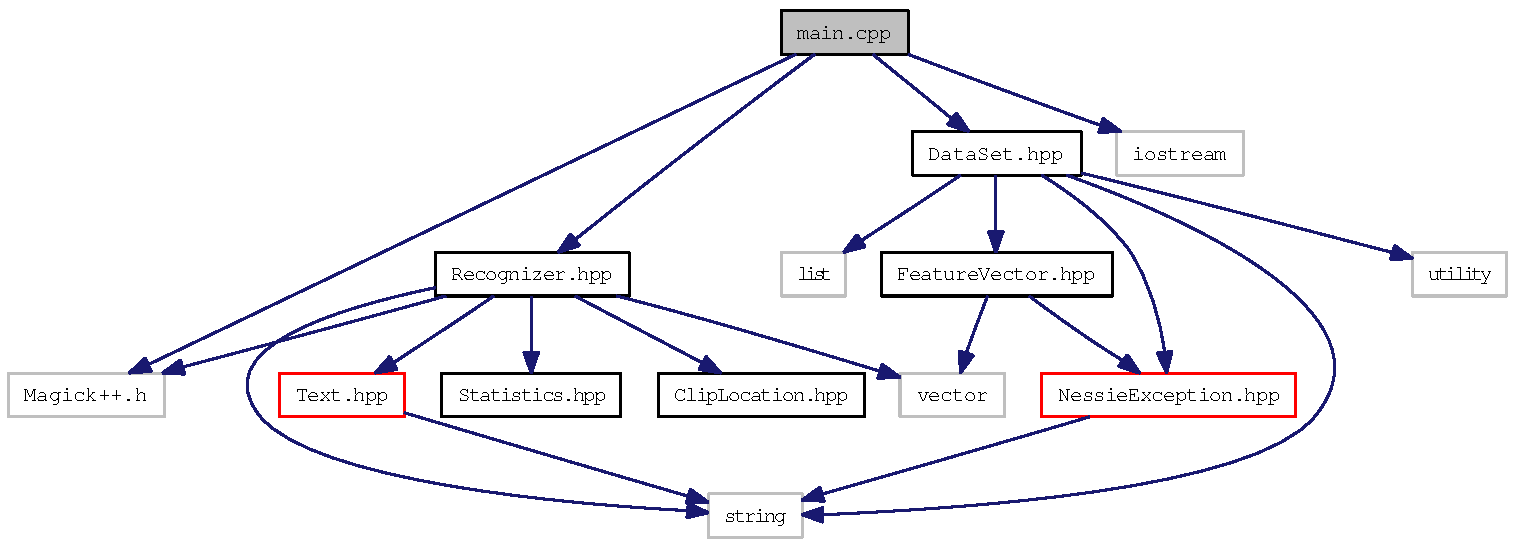
\includegraphics[width=282pt]{main_8cpp__incl}
\end{center}
\end{figure}
\subsection*{Functions}
\begin{CompactItemize}
\item 
int \hyperlink{main_8cpp_bf9e6b7e6f15df4b525a2e7705ba3089}{main} (int argc, char const $\ast$argv\mbox{[}$\,$\mbox{]})
\end{CompactItemize}


\subsection{Function Documentation}
\hypertarget{main_8cpp_bf9e6b7e6f15df4b525a2e7705ba3089}{
\index{main.cpp@{main.cpp}!main@{main}}
\index{main@{main}!main.cpp@{main.cpp}}
\subsubsection[main]{\setlength{\rightskip}{0pt plus 5cm}int main (int {\em argc}, \/  char const $\ast$ {\em argv}\mbox{[}$\,$\mbox{]})}}
\label{main_8cpp_bf9e6b7e6f15df4b525a2e7705ba3089}


\begin{Desc}
\item[\hyperlink{todo__todo000001}{Todo}]Improve the performance of \hyperlink{class_segmenter_684df74b0e810a837669823c47b6ed87}{Segmenter::exploreSeedNeighbourhood()} by developing a non-recursive approach \end{Desc}
\begin{Desc}
\item[\hyperlink{todo__todo000001}{Todo}]Develop a method to sort the list of shapes according to their position in text. \end{Desc}
\begin{Desc}
\item[\hyperlink{todo__todo000001}{Todo}]Change the \hyperlink{class_clip_454ff6070d0918e56a09a3f28ff430c3}{Clip::setPixelGrayLevel()} and \hyperlink{class_clip_85d16f086803860fae205c48161a3c38}{Clip::getPixelGrayLevel} methods for operator() overloading. \end{Desc}
\begin{Desc}
\item[\hyperlink{todo__todo000001}{Todo}]Overload operator+ for the class \hyperlink{class_text}{Text}. \end{Desc}
\begin{Desc}
\item[\hyperlink{todo__todo000001}{Todo}]Overload operator- and operator+ for the class \hyperlink{class_statistics}{Statistics}.\end{Desc}
\begin{Desc}
\item[Parameters:]
\begin{description}
\item[{\em argc}]Number of command line arguments \item[{\em argv}]Command line arguments\end{description}
\end{Desc}
\begin{Desc}
\item[Author:]Eliezer Talón (\href{mailto:elitalon@gmail.com}{\tt elitalon@gmail.com}) \end{Desc}
\begin{Desc}
\item[Date:]2008-10-16 \end{Desc}


Definition at line 26 of file main.cpp.